Before assessing the physical correctness of the ID regression models, the physical correctness of the Reference model was first be assessed. Standard manoeuvring model tests were used for this purpose. As a first step, total forces and moments from the model test were estimates with inverse dynamics (see \autoref{sec:inverse_dynamics}). These forces were compared with corresponding forces predicted with the Reference model. 
\autoref{fig:VCT_regression_ID} shows such a comparison for a zigzag20/20 model test. The first graph shows the rudder signal $\delta$ together with drift angle $\beta$ and yaw rate $r$. A comparison of sway force $Y_D$ and yawing moment $N_D$ are shown in the other two graphs. The forces and moments predicted with the Reference model were in reasonable agreement with the forces from the experiment. There were small deviations, where the Reference model over predicted the forces and moments in the peaks -- in the ends of the counter rudder excitations. 
The predicted force signals had the same general shape as the experimental forces, which implies that the Reference model captures most of the essential physics involved in the experiment.
Comparisons with the other tests are summarized as the mean average error in \autoref{tab:reference_model_mean_average_error}. The other zigzag20/20 has about the same error as the one in \autoref{fig:VCT_regression_ID}. For the zigzag10/10 tests, the errors were smaller, which was also the case for the yaw rate and reference speed tests.
\begin{figure}[h!]
    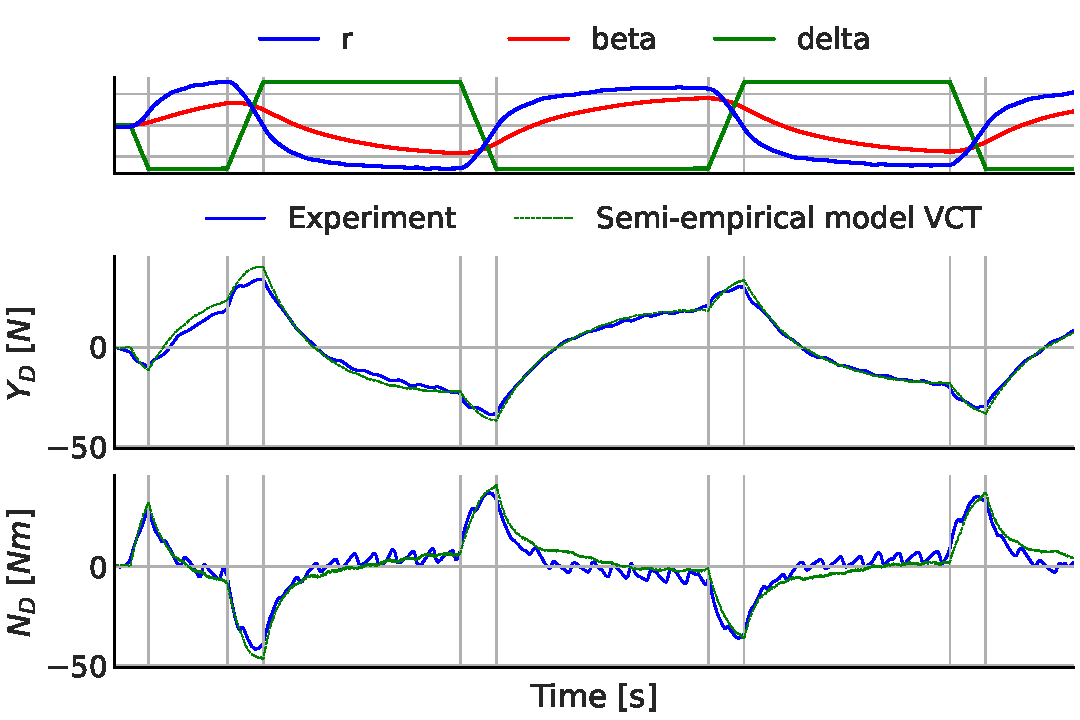
\includegraphics[width=\columnwidth]{figures/result_VCT_regression.VCT_regression_ID.pdf}
    \caption{Comparison of the total forces acting on the ship: predicted with the Semi-empirical VCT model, and the corresponding values from a zigzag20/20 test estimated with inverse dynamics.}
    \label{fig:VCT_regression_ID}
\end{figure}

\begin{table}[h!]
    \centering
    \caption{Mean average error of the Reference model compared to the inverse dynamics forces from the models tests.}
    \label{tab:reference_model_mean_average_error}
    \pgfplotstabletypeset[col sep=comma,fixed,fixed zerofill,precision=1,column type=l,
    %columns={Test type,$u$,$v$,$r$,$\delta$,$\eta_0$},
    columns/Description/.style={string type, column type=l},
    columns/V/.style={column name=$V$ $[m/s]$,fixed, precision=2, column type=l},
    ]{"tables/result_VCT_regression.reference_model_mean_average_error.csv"}
\end{table}